\subsection{UC27: Gestione dei prodotti}
        \label{sec:UC27}
        \begin{figure}[!ht]
            \caption{Diagramma di UC27: Gestione dei prodotti}
            \vspace{10px}
            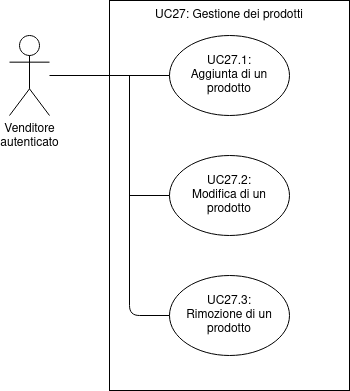
\includegraphics[scale=0.5]{../../../Images/AnalisiRequisiti/UC27}
            \centering
        \end{figure}
        \begin{itemize}
            \item \textbf{Descrizione:} sezione per il venditore, dove può gestire i prodotti del negozio;
            \item \textbf{Attore Primario:} venditore autenticato;
            \item \textbf{Precondizione:} il venditore si trova in una qualsiasi pagina del negozio;
            \item \textbf{Input:} il venditore preme il bottone per entrare in questa sezione;
            \item \textbf{Postcondizione:} il venditore ha completato le modifiche ai prodotti desiderati;
            \item \textbf{Scenario Principale:} 
                \begin{itemize}
                    \item il venditore si trova nella pagina per la gestione del negozio;
                    \item può decidere se aggiungere un nuovo prodotto, modificarne o rimuoverne uno già presente;
                    \item una volta terminato applica le modifiche
                \end{itemize}
        \end{itemize}
        \subsubsection{UC27.1: Aggiunta di un prodotto}
        \begin{itemize}
            \item \textbf{Descrizione:} sezione per aggiungere un prodotto nel negozio;
            \item \textbf{Attore Primario:} venditore autenticato;
            \item \textbf{Precondizione:} il venditore si trova nella sezione per gestire i prodotti (\hyperref[sec:UC27]{\underline{UC27}});
            \item \textbf{Input:} il venditore inserisce tutti i dati relativi al prodotto da inserire;
            \item \textbf{Postcondizione:} il prodotto è aggiunto e i clienti possono trovarlo nel negozio;
            \item \textbf{Scenario Principale:} 
                \begin{itemize}
                    \item il venditore si trova nella sezione per gestire i prodotti;
                    \item il venditore decide di aggiungere un nuovo prodotto ed entra in questa sezione;
                    \item inserisce tutti i dati richiesti (nome, descrizione, prezzo ecc.);
                    \item conferma l'aggiunta e il prodotto è disponibile nel negozio.
                \end{itemize}
        \end{itemize}
        \subsubsection{UC27.2: Modifica di un prodotto}
        \begin{itemize}
            \item \textbf{Descrizione:} sezione per modificare un prodotto del negozio;
            \item \textbf{Attore Primario:} venditore autenticato;
            \item \textbf{Precondizione:} il venditore si trova nella sezione per gestire i prodotti (\hyperref[sec:UC27]{\underline{UC27}});
            \item \textbf{Input:} il venditore modifica i dati che ritiene opportuni relativi al prodotto da modificare;
            \item \textbf{Postcondizione:} il prodotto è stato modificato;
            \item \textbf{Scenario Principale:} 
                \begin{itemize}
                    \item il venditore si trova nella sezione per gestire i prodotti;
                    \item il venditore decide di modificare un prodotto ed entra in questa sezione;
                    \item modifica i dati che preferisce;
                    \item conferma le modifiche.
                \end{itemize}
        \end{itemize}
        \subsubsubsection{UC27.3: Rimozione di un prodotto}
        \begin{itemize}
            \item \textbf{Descrizione:} sezione per rimuovere un prodotto dal negozio;
            \item \textbf{Attore Primario:} venditore autenticato;
            \item \textbf{Precondizione:} il venditore si trova nella sezione per gestire i prodotti (\hyperref[sec:UC27]{\underline{UC27}});
            \item \textbf{Input:} il venditore sceglie il prodotto da eliminare;
            \item \textbf{Postcondizione:} il prodotto è stato rimosso dal negozio;
            \item \textbf{Scenario Principale:} 
                \begin{itemize}
                    \item il venditore si trova nella sezione per gestire i prodotti;
                    \item il venditore decide di rimuovere un prodotto dal negozio;
                    \item conferma;
                    \item il prodotto non è più visibile nel negozio.
                \end{itemize}
        \end{itemize}